\documentclass[10pt,a4paper]{article}
\usepackage{tikz}
\usetikzlibrary{positioning}
\usetikzlibrary{shapes.misc}
\begin{document}
				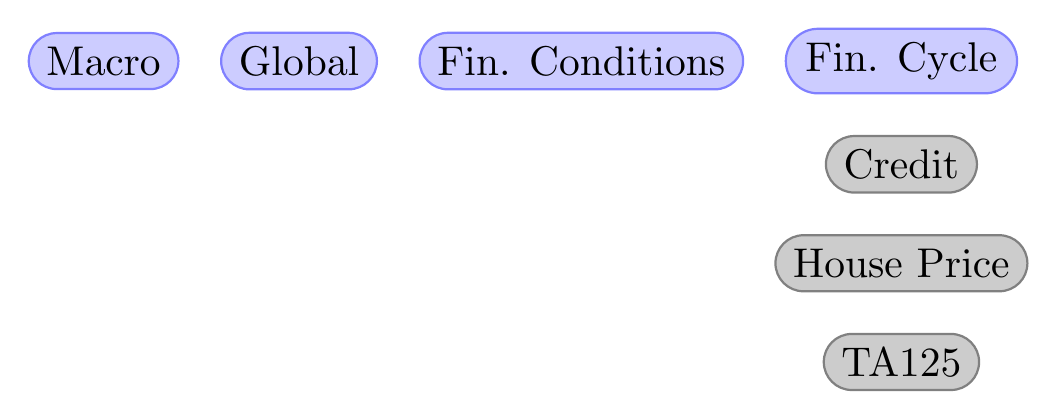
\begin{tikzpicture}
	[nodestyle/.style={rounded rectangle,draw=blue!50,fill=blue!20,thick, scale=1.5},
	greynodestyle/.style={rounded rectangle,draw=black!50,fill=black!20,thick, scale=1.5}
	]
	
	%Set params
	\def\hor_dist{0.5}
	\def\ver_dist{0.5}
	
	\node(Macro)[nodestyle]{Macro};			
	\node(Global)[nodestyle, right  = \hor_dist cm of Macro]{Global};			
	\node(FinCon)[nodestyle, right  = \hor_dist cm of Global]{Fin. Conditions};			
	\node(FinCycle)[nodestyle, right  = \hor_dist cm of FinCon]{Fin. Cycle};
	
	%Fin cycle
	\node(Credit)[greynodestyle, below = \ver_dist cm of FinCycle] {Credit};
	\node(House)[greynodestyle, below = \ver_dist cm of Credit] {House Price};
	\node(TA)[greynodestyle, below = \ver_dist cm of House] {TA125};
	
	\end{tikzpicture}

\end{document}